\documentclass{beamer}
\usepackage[dutch]{babel}
\usepackage{graphicx}
\usepackage{url}
\usepackage{fancyvrb}

\usepackage{fancyvrb}
\usepackage{color}

\makeatletter
\def\PY@reset{\let\PY@it=\relax \let\PY@bf=\relax%
    \let\PY@ul=\relax \let\PY@tc=\relax%
    \let\PY@bc=\relax \let\PY@ff=\relax}
\def\PY@tok#1{\csname PY@tok@#1\endcsname}
\def\PY@toks#1+{\ifx\relax#1\empty\else%
    \PY@tok{#1}\expandafter\PY@toks\fi}
\def\PY@do#1{\PY@bc{\PY@tc{\PY@ul{%
    \PY@it{\PY@bf{\PY@ff{#1}}}}}}}
\def\PY#1#2{\PY@reset\PY@toks#1+\relax+\PY@do{#2}}

\def\PY@tok@gd{\def\PY@tc##1{\textcolor[rgb]{0.63,0.00,0.00}{##1}}}
\def\PY@tok@gu{\let\PY@bf=\textbf\def\PY@tc##1{\textcolor[rgb]{0.50,0.00,0.50}{##1}}}
\def\PY@tok@gt{\def\PY@tc##1{\textcolor[rgb]{0.00,0.25,0.82}{##1}}}
\def\PY@tok@gs{\let\PY@bf=\textbf}
\def\PY@tok@gr{\def\PY@tc##1{\textcolor[rgb]{1.00,0.00,0.00}{##1}}}
\def\PY@tok@cm{\let\PY@it=\textit\def\PY@tc##1{\textcolor[rgb]{0.25,0.50,0.50}{##1}}}
\def\PY@tok@vg{\def\PY@tc##1{\textcolor[rgb]{0.10,0.09,0.49}{##1}}}
\def\PY@tok@m{\def\PY@tc##1{\textcolor[rgb]{0.40,0.40,0.40}{##1}}}
\def\PY@tok@mh{\def\PY@tc##1{\textcolor[rgb]{0.40,0.40,0.40}{##1}}}
\def\PY@tok@go{\def\PY@tc##1{\textcolor[rgb]{0.50,0.50,0.50}{##1}}}
\def\PY@tok@ge{\let\PY@it=\textit}
\def\PY@tok@vc{\def\PY@tc##1{\textcolor[rgb]{0.10,0.09,0.49}{##1}}}
\def\PY@tok@il{\def\PY@tc##1{\textcolor[rgb]{0.40,0.40,0.40}{##1}}}
\def\PY@tok@cs{\let\PY@it=\textit\def\PY@tc##1{\textcolor[rgb]{0.25,0.50,0.50}{##1}}}
\def\PY@tok@cp{\def\PY@tc##1{\textcolor[rgb]{0.74,0.48,0.00}{##1}}}
\def\PY@tok@gi{\def\PY@tc##1{\textcolor[rgb]{0.00,0.63,0.00}{##1}}}
\def\PY@tok@gh{\let\PY@bf=\textbf\def\PY@tc##1{\textcolor[rgb]{0.00,0.00,0.50}{##1}}}
\def\PY@tok@ni{\let\PY@bf=\textbf\def\PY@tc##1{\textcolor[rgb]{0.60,0.60,0.60}{##1}}}
\def\PY@tok@nl{\def\PY@tc##1{\textcolor[rgb]{0.63,0.63,0.00}{##1}}}
\def\PY@tok@nn{\let\PY@bf=\textbf\def\PY@tc##1{\textcolor[rgb]{0.00,0.00,1.00}{##1}}}
\def\PY@tok@no{\def\PY@tc##1{\textcolor[rgb]{0.53,0.00,0.00}{##1}}}
\def\PY@tok@na{\def\PY@tc##1{\textcolor[rgb]{0.49,0.56,0.16}{##1}}}
\def\PY@tok@nb{\def\PY@tc##1{\textcolor[rgb]{0.00,0.50,0.00}{##1}}}
\def\PY@tok@nc{\let\PY@bf=\textbf\def\PY@tc##1{\textcolor[rgb]{0.00,0.00,1.00}{##1}}}
\def\PY@tok@nd{\def\PY@tc##1{\textcolor[rgb]{0.67,0.13,1.00}{##1}}}
\def\PY@tok@ne{\let\PY@bf=\textbf\def\PY@tc##1{\textcolor[rgb]{0.82,0.25,0.23}{##1}}}
\def\PY@tok@nf{\def\PY@tc##1{\textcolor[rgb]{0.00,0.00,1.00}{##1}}}
\def\PY@tok@si{\let\PY@bf=\textbf\def\PY@tc##1{\textcolor[rgb]{0.73,0.40,0.53}{##1}}}
\def\PY@tok@s2{\def\PY@tc##1{\textcolor[rgb]{0.73,0.13,0.13}{##1}}}
\def\PY@tok@vi{\def\PY@tc##1{\textcolor[rgb]{0.10,0.09,0.49}{##1}}}
\def\PY@tok@nt{\let\PY@bf=\textbf\def\PY@tc##1{\textcolor[rgb]{0.00,0.50,0.00}{##1}}}
\def\PY@tok@nv{\def\PY@tc##1{\textcolor[rgb]{0.10,0.09,0.49}{##1}}}
\def\PY@tok@s1{\def\PY@tc##1{\textcolor[rgb]{0.73,0.13,0.13}{##1}}}
\def\PY@tok@sh{\def\PY@tc##1{\textcolor[rgb]{0.73,0.13,0.13}{##1}}}
\def\PY@tok@sc{\def\PY@tc##1{\textcolor[rgb]{0.73,0.13,0.13}{##1}}}
\def\PY@tok@sx{\def\PY@tc##1{\textcolor[rgb]{0.00,0.50,0.00}{##1}}}
\def\PY@tok@bp{\def\PY@tc##1{\textcolor[rgb]{0.00,0.50,0.00}{##1}}}
\def\PY@tok@c1{\let\PY@it=\textit\def\PY@tc##1{\textcolor[rgb]{0.25,0.50,0.50}{##1}}}
\def\PY@tok@kc{\let\PY@bf=\textbf\def\PY@tc##1{\textcolor[rgb]{0.00,0.50,0.00}{##1}}}
\def\PY@tok@c{\let\PY@it=\textit\def\PY@tc##1{\textcolor[rgb]{0.25,0.50,0.50}{##1}}}
\def\PY@tok@mf{\def\PY@tc##1{\textcolor[rgb]{0.40,0.40,0.40}{##1}}}
\def\PY@tok@err{\def\PY@bc##1{\fcolorbox[rgb]{1.00,0.00,0.00}{1,1,1}{##1}}}
\def\PY@tok@kd{\let\PY@bf=\textbf\def\PY@tc##1{\textcolor[rgb]{0.00,0.50,0.00}{##1}}}
\def\PY@tok@ss{\def\PY@tc##1{\textcolor[rgb]{0.10,0.09,0.49}{##1}}}
\def\PY@tok@sr{\def\PY@tc##1{\textcolor[rgb]{0.73,0.40,0.53}{##1}}}
\def\PY@tok@mo{\def\PY@tc##1{\textcolor[rgb]{0.40,0.40,0.40}{##1}}}
\def\PY@tok@kn{\let\PY@bf=\textbf\def\PY@tc##1{\textcolor[rgb]{0.00,0.50,0.00}{##1}}}
\def\PY@tok@mi{\def\PY@tc##1{\textcolor[rgb]{0.40,0.40,0.40}{##1}}}
\def\PY@tok@gp{\let\PY@bf=\textbf\def\PY@tc##1{\textcolor[rgb]{0.00,0.00,0.50}{##1}}}
\def\PY@tok@o{\def\PY@tc##1{\textcolor[rgb]{0.40,0.40,0.40}{##1}}}
\def\PY@tok@kr{\let\PY@bf=\textbf\def\PY@tc##1{\textcolor[rgb]{0.00,0.50,0.00}{##1}}}
\def\PY@tok@s{\def\PY@tc##1{\textcolor[rgb]{0.73,0.13,0.13}{##1}}}
\def\PY@tok@kp{\def\PY@tc##1{\textcolor[rgb]{0.00,0.50,0.00}{##1}}}
\def\PY@tok@w{\def\PY@tc##1{\textcolor[rgb]{0.73,0.73,0.73}{##1}}}
\def\PY@tok@kt{\def\PY@tc##1{\textcolor[rgb]{0.69,0.00,0.25}{##1}}}
\def\PY@tok@ow{\let\PY@bf=\textbf\def\PY@tc##1{\textcolor[rgb]{0.67,0.13,1.00}{##1}}}
\def\PY@tok@sb{\def\PY@tc##1{\textcolor[rgb]{0.73,0.13,0.13}{##1}}}
\def\PY@tok@k{\let\PY@bf=\textbf\def\PY@tc##1{\textcolor[rgb]{0.00,0.50,0.00}{##1}}}
\def\PY@tok@se{\let\PY@bf=\textbf\def\PY@tc##1{\textcolor[rgb]{0.73,0.40,0.13}{##1}}}
\def\PY@tok@sd{\let\PY@it=\textit\def\PY@tc##1{\textcolor[rgb]{0.73,0.13,0.13}{##1}}}

\def\PYZbs{\char`\\}
\def\PYZus{\char`\_}
\def\PYZob{\char`\{}
\def\PYZcb{\char`\}}
\def\PYZca{\char`\^}
% for compatibility with earlier versions
\def\PYZat{@}
\def\PYZlb{[}
\def\PYZrb{]}
\makeatother
   % Pygmentize preamble

\title{Perceptual Hashes}
\subtitle{Een inleiding}
\author{Koen Crolla}
\date{24 mei 2012}

\begin{document}

{\logo{
\includegraphics[scale=.2]{LogoGT.png}} \maketitle}

\begin{frame}
  \frametitle{Vooraf}

  Alle code, afbeeldingen, slides:

  \centering

  \LARGE \url{https://github.com/Cairnarvon/phash-presentation}

\end{frame}


%% Introduction

\begin{frame}
  \frametitle{Probleem}

  We hebben een afbeelding:

  \centering

  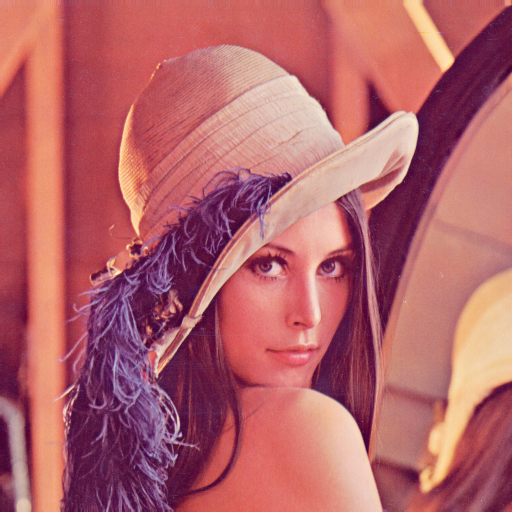
\includegraphics[height=2in]{../target.png}

\end{frame}

\begin{frame}
  ... en een hoeveelheid andere afbeeldingen:

  \centering

  \begin{tabular}{cccccccc}
    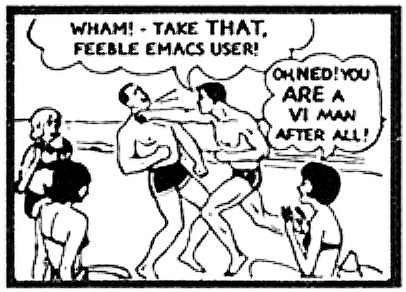
\includegraphics[height=.3in,width=.3in,keepaspectratio]{../images/01.jpg} &
    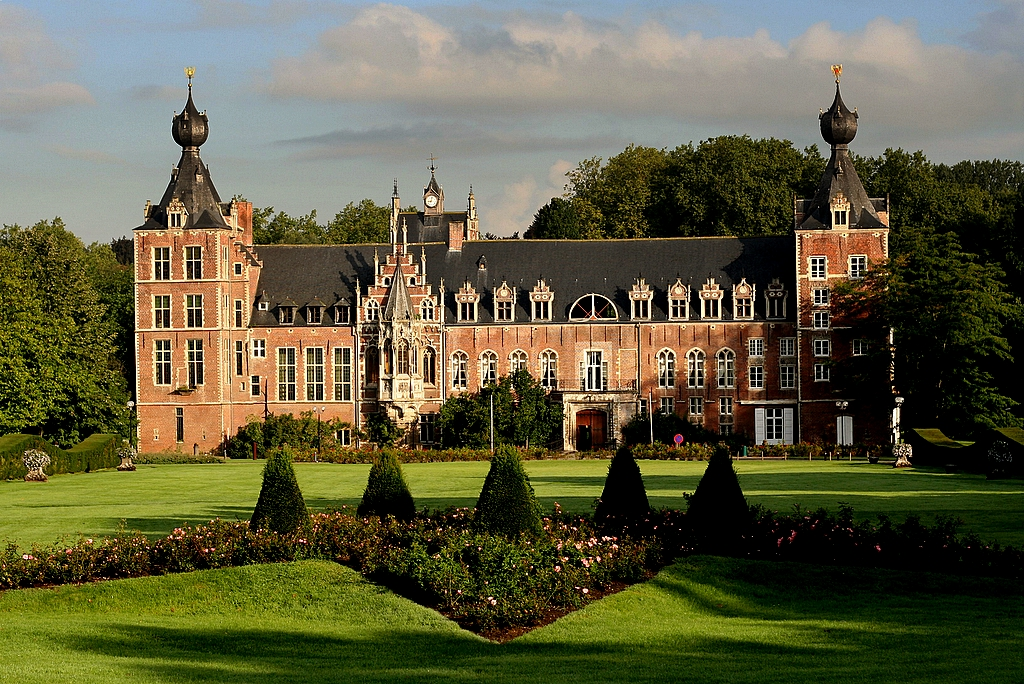
\includegraphics[height=.3in,width=.3in,keepaspectratio]{../images/02.jpg} &
    
\includegraphics[height=.3in,width=.3in,keepaspectratio]{../images/03.jpg} &
    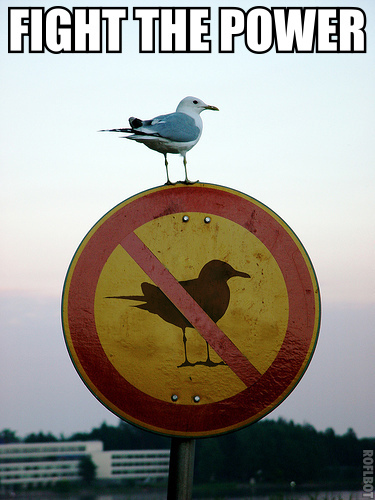
\includegraphics[height=.3in,width=.3in,keepaspectratio]{../images/04.jpg} &
    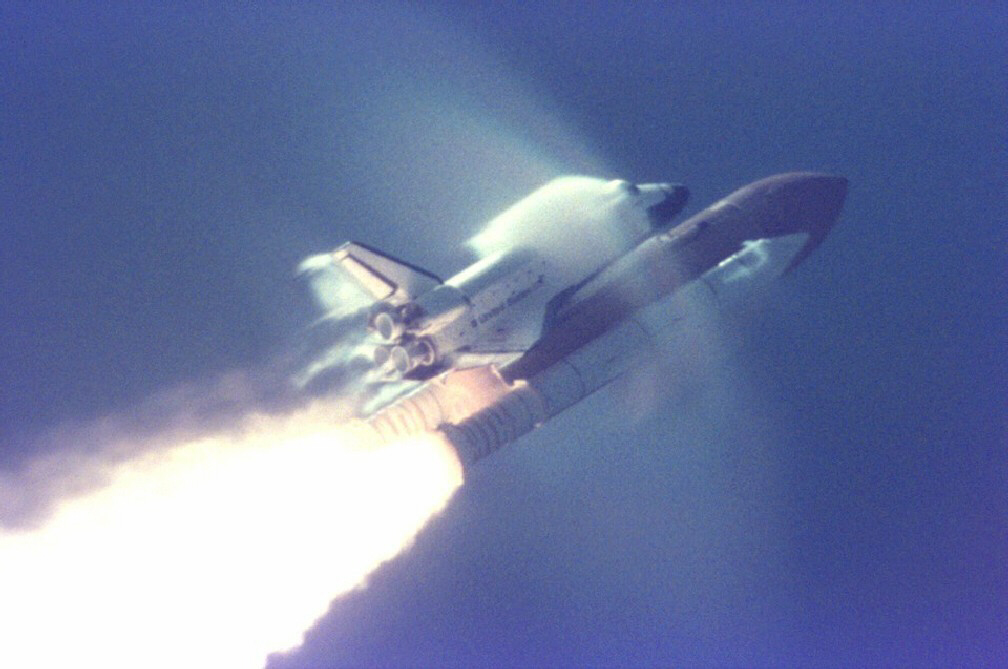
\includegraphics[height=.3in,width=.3in,keepaspectratio]{../images/05.jpg} &
    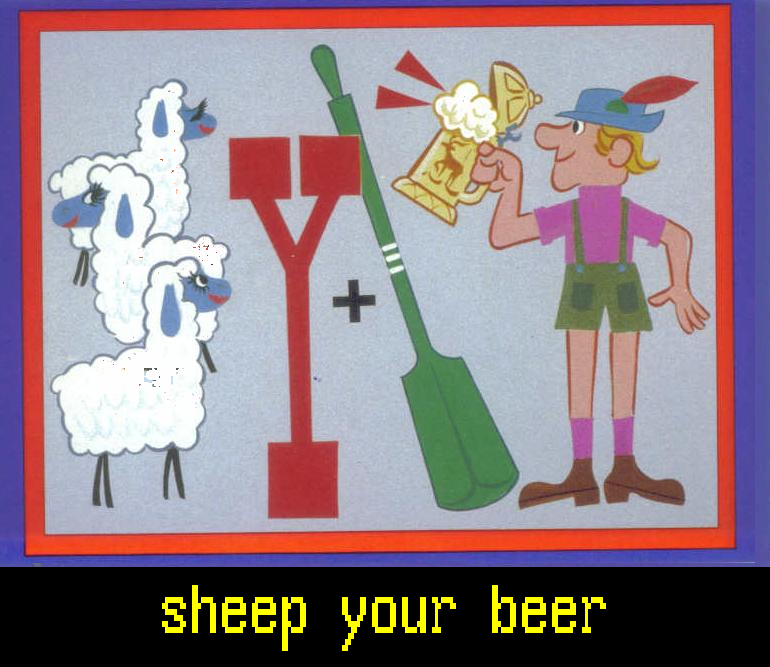
\includegraphics[height=.3in,width=.3in,keepaspectratio]{../images/06.png} &
    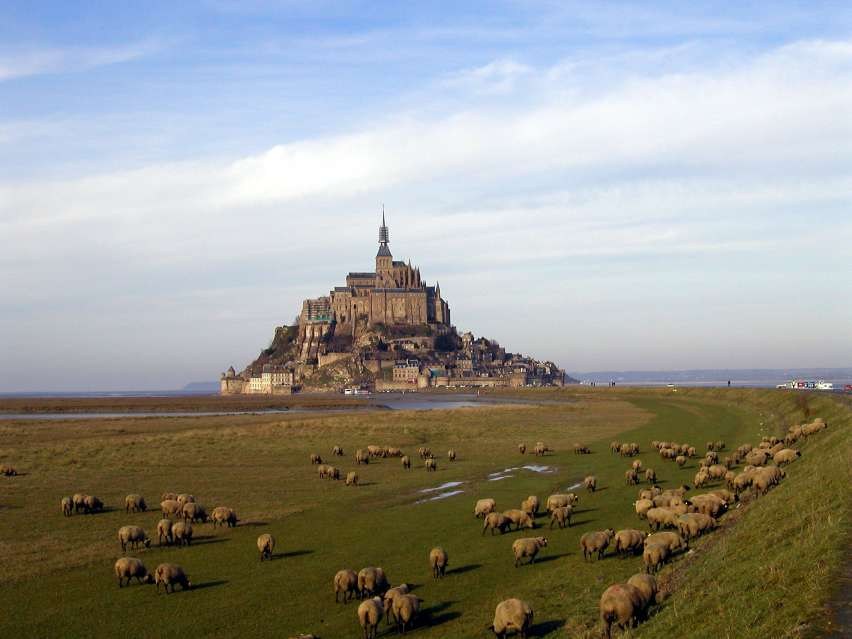
\includegraphics[height=.3in,width=.3in,keepaspectratio]{../images/07.jpg} &
    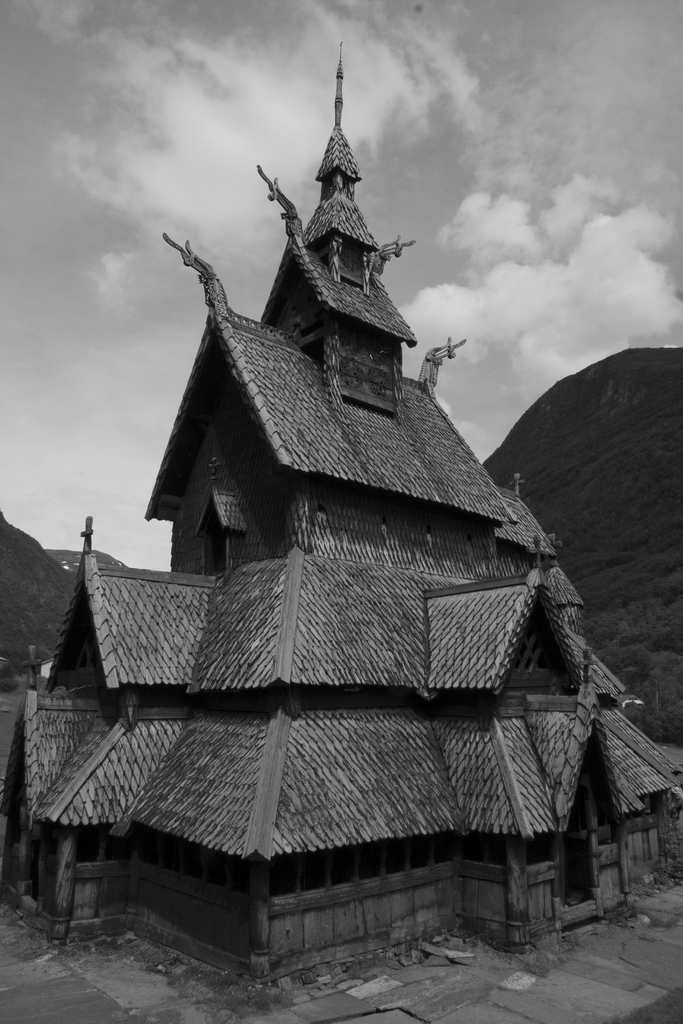
\includegraphics[height=.3in,width=.3in,keepaspectratio]{../images/08.jpg} \\
    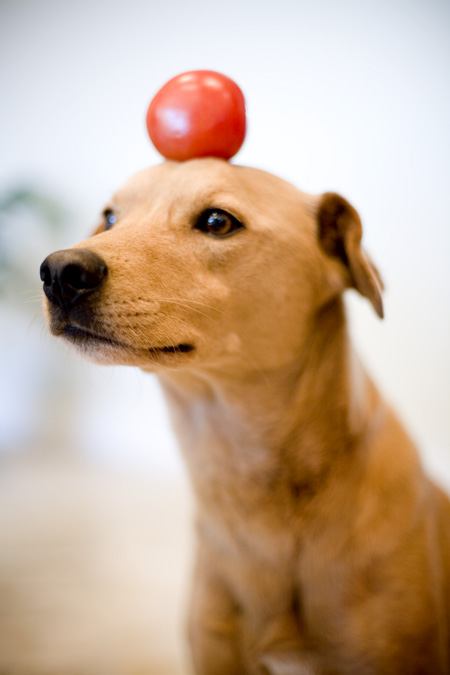
\includegraphics[height=.3in,width=.3in,keepaspectratio]{../images/09.jpg} &
    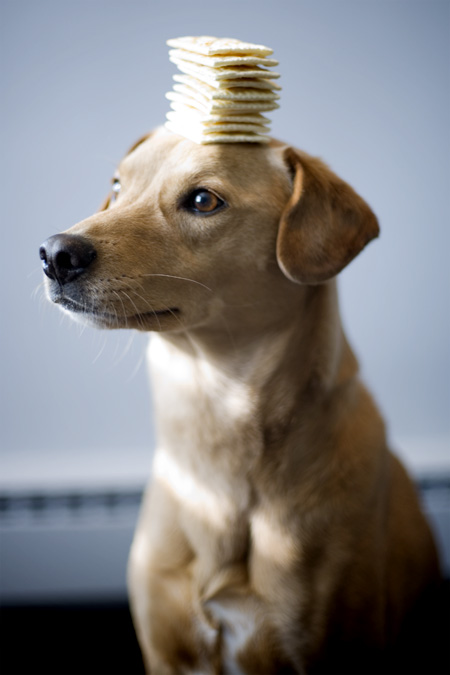
\includegraphics[height=.3in,width=.3in,keepaspectratio]{../images/10.jpg} &
    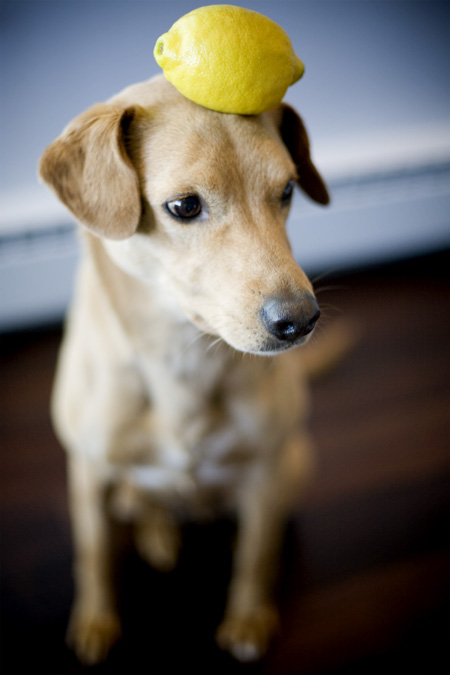
\includegraphics[height=.3in,width=.3in,keepaspectratio]{../images/11.jpg} &
    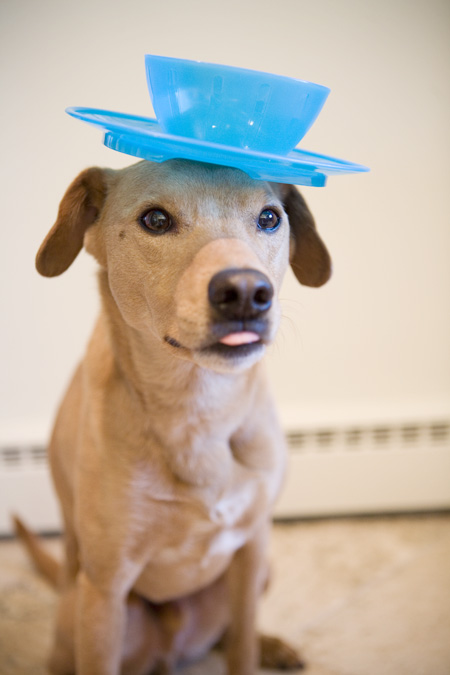
\includegraphics[height=.3in,width=.3in,keepaspectratio]{../images/12.jpg} &
    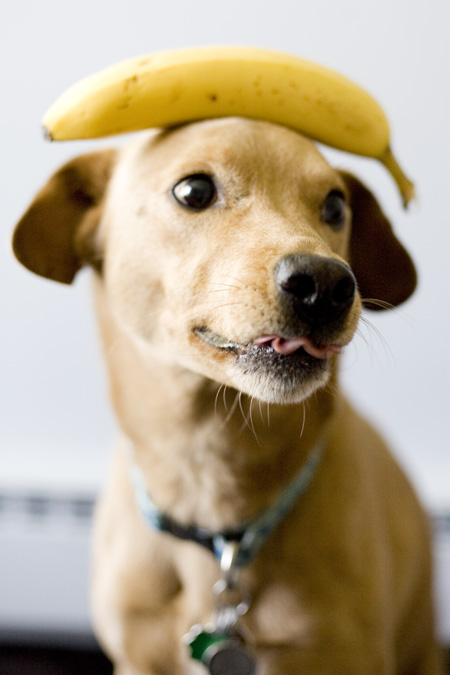
\includegraphics[height=.3in,width=.3in,keepaspectratio]{../images/13.jpg} &
    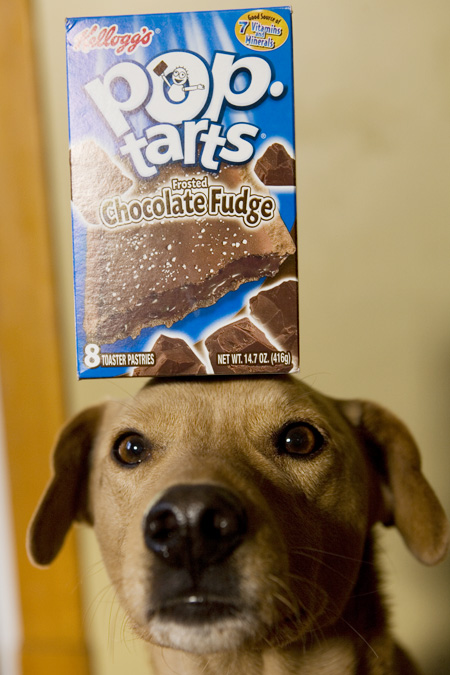
\includegraphics[height=.3in,width=.3in,keepaspectratio]{../images/14.jpg} &
    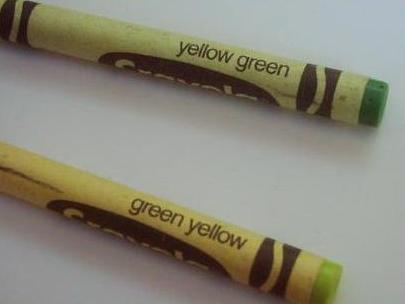
\includegraphics[height=.3in,width=.3in,keepaspectratio]{../images/15.jpg} &
    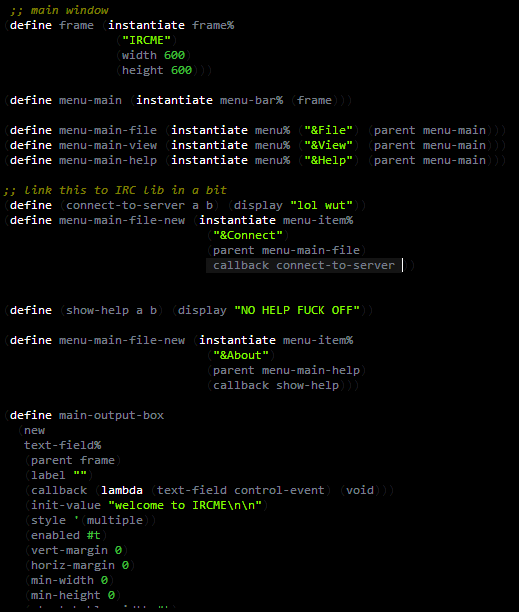
\includegraphics[height=.3in,width=.3in,keepaspectratio]{../images/16.png} \\ 
    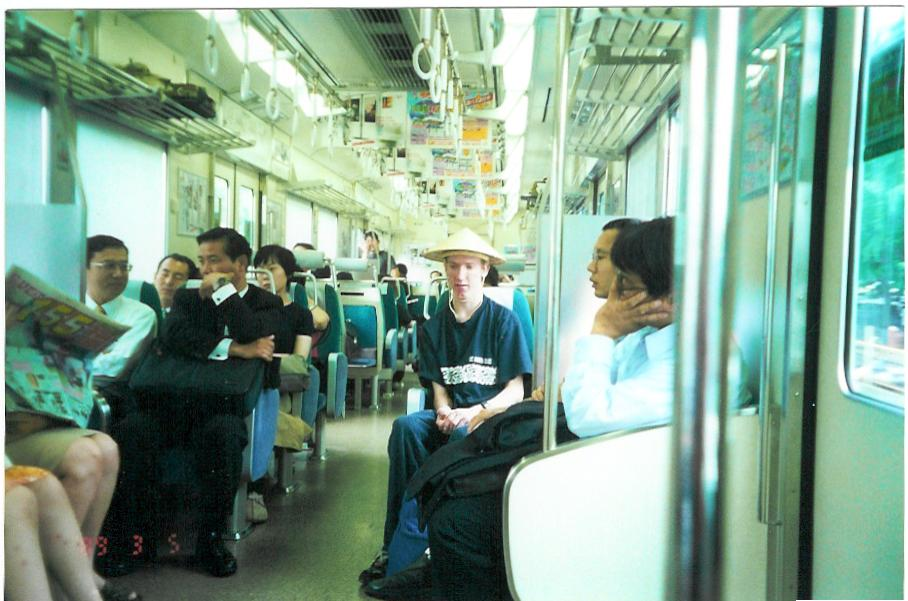
\includegraphics[height=.3in,width=.3in,keepaspectratio]{../images/17.jpg} &
    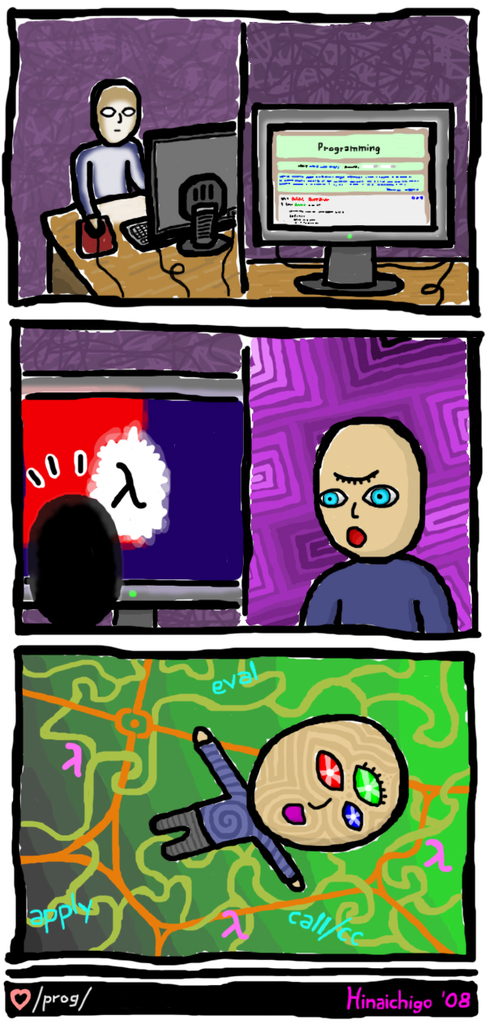
\includegraphics[height=.3in,width=.3in,keepaspectratio]{../images/18.jpg} &
    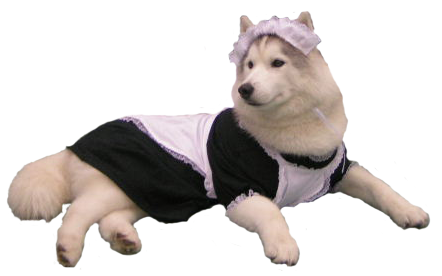
\includegraphics[height=.3in,width=.3in,keepaspectratio]{../images/19.png} &
    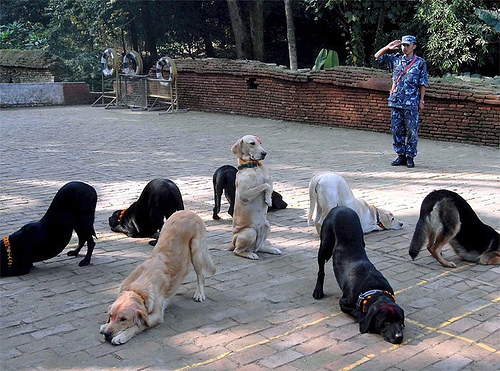
\includegraphics[height=.3in,width=.3in,keepaspectratio]{../images/20.jpg} &
    
\includegraphics[height=.3in,width=.3in,keepaspectratio]{../images/21.png} &
    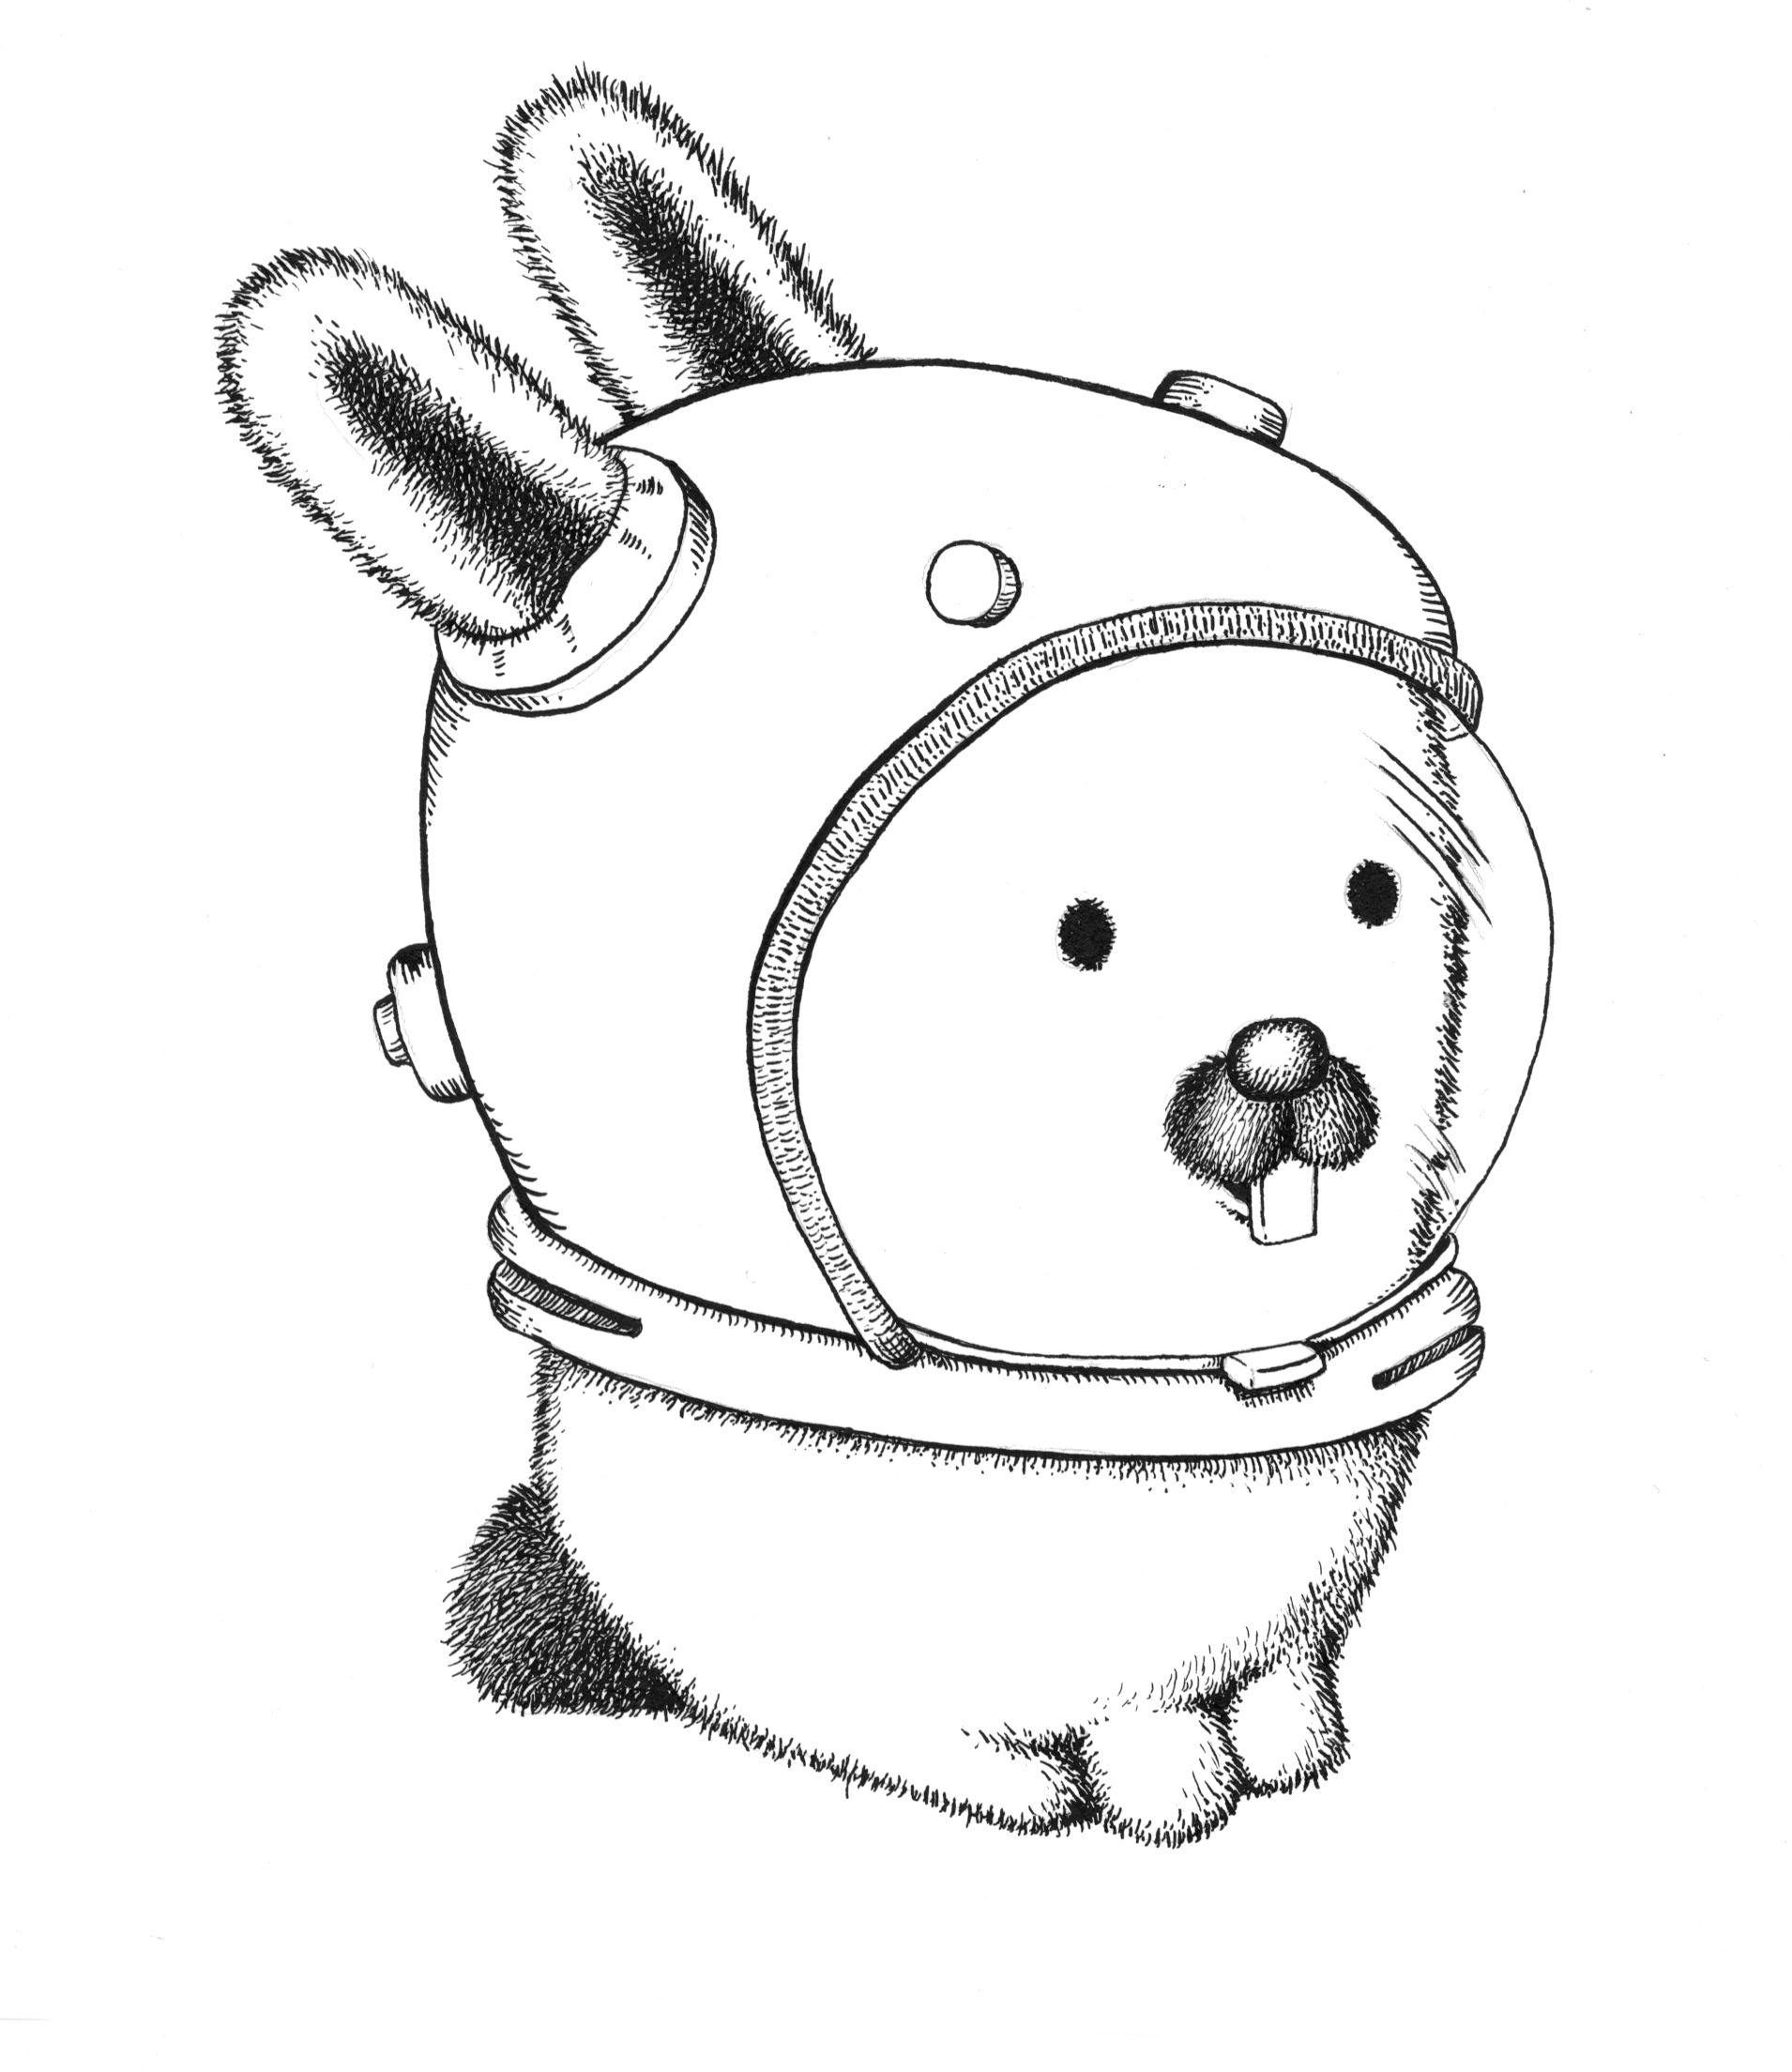
\includegraphics[height=.3in,width=.3in,keepaspectratio]{../images/22.jpg} &
    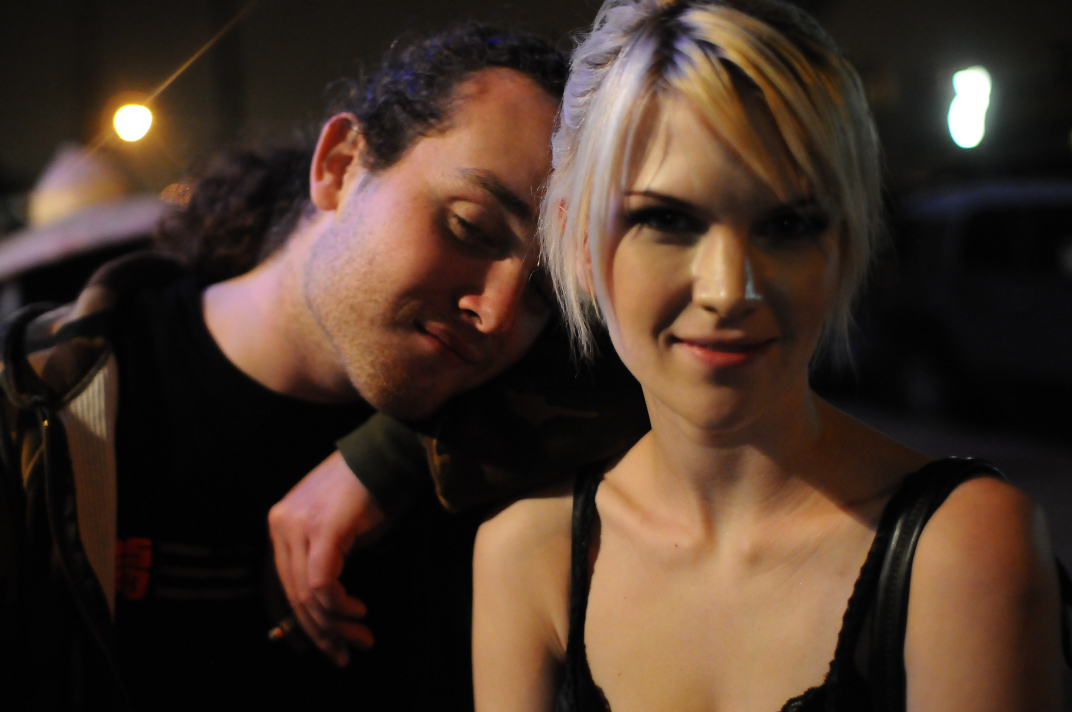
\includegraphics[height=.3in,width=.3in,keepaspectratio]{../images/23.jpg} &
    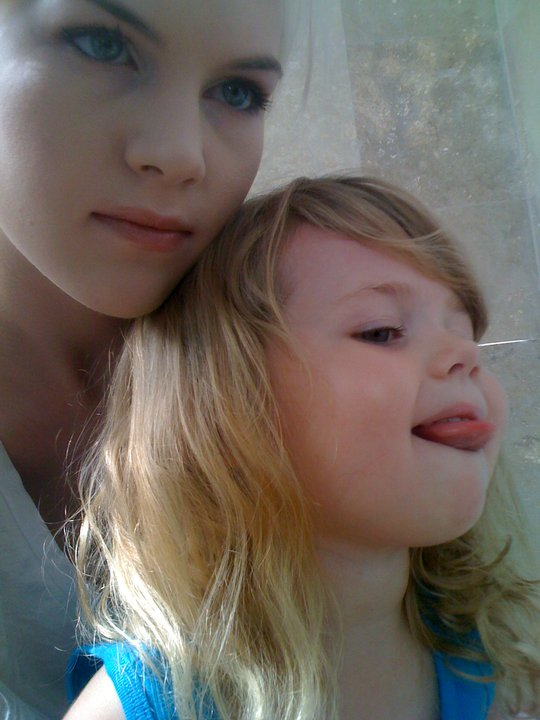
\includegraphics[height=.3in,width=.3in,keepaspectratio]{../images/24.jpg} \\
    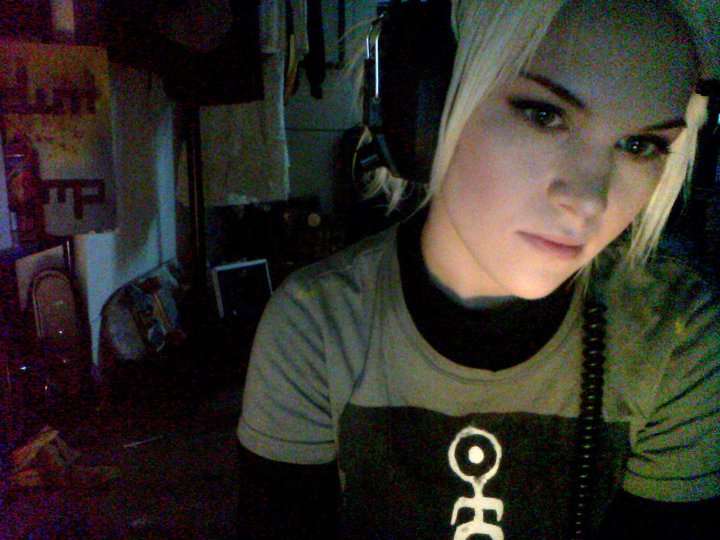
\includegraphics[height=.3in,width=.3in,keepaspectratio]{../images/25.jpg} &
    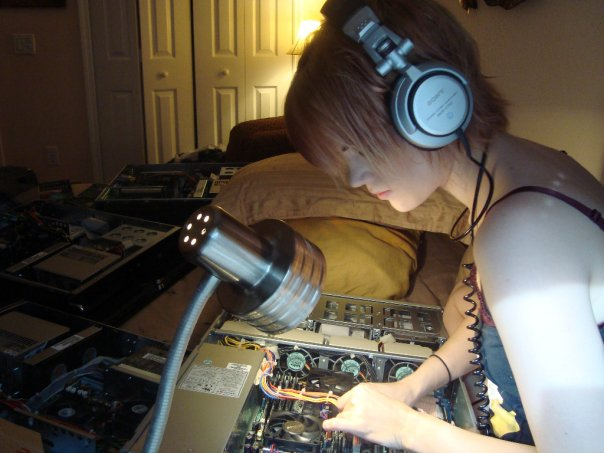
\includegraphics[height=.3in,width=.3in,keepaspectratio]{../images/26.jpg} &
    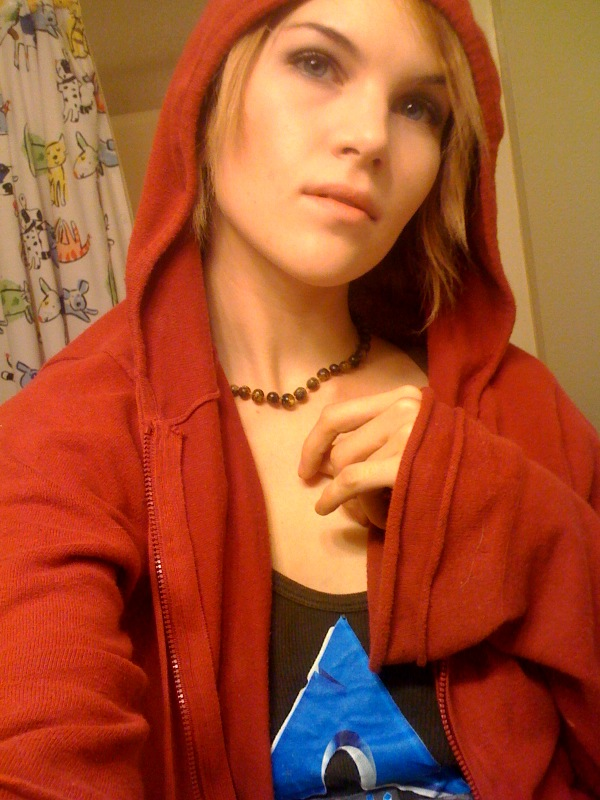
\includegraphics[height=.3in,width=.3in,keepaspectratio]{../images/27.jpg} &
    
\includegraphics[height=.3in,width=.3in,keepaspectratio]{../images/28.jpg} &
    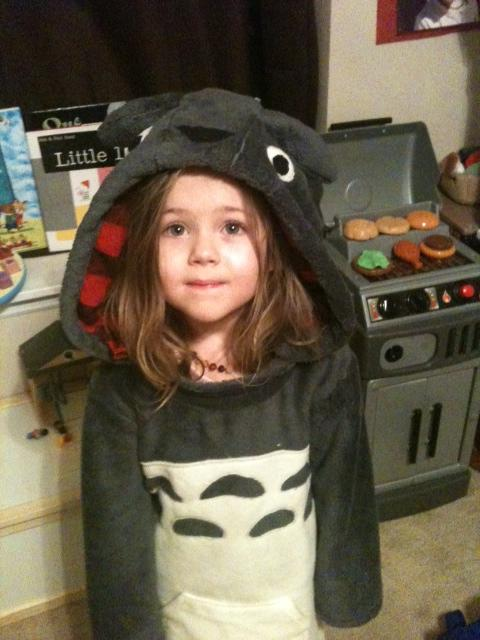
\includegraphics[height=.3in,width=.3in,keepaspectratio]{../images/29.jpg} &
    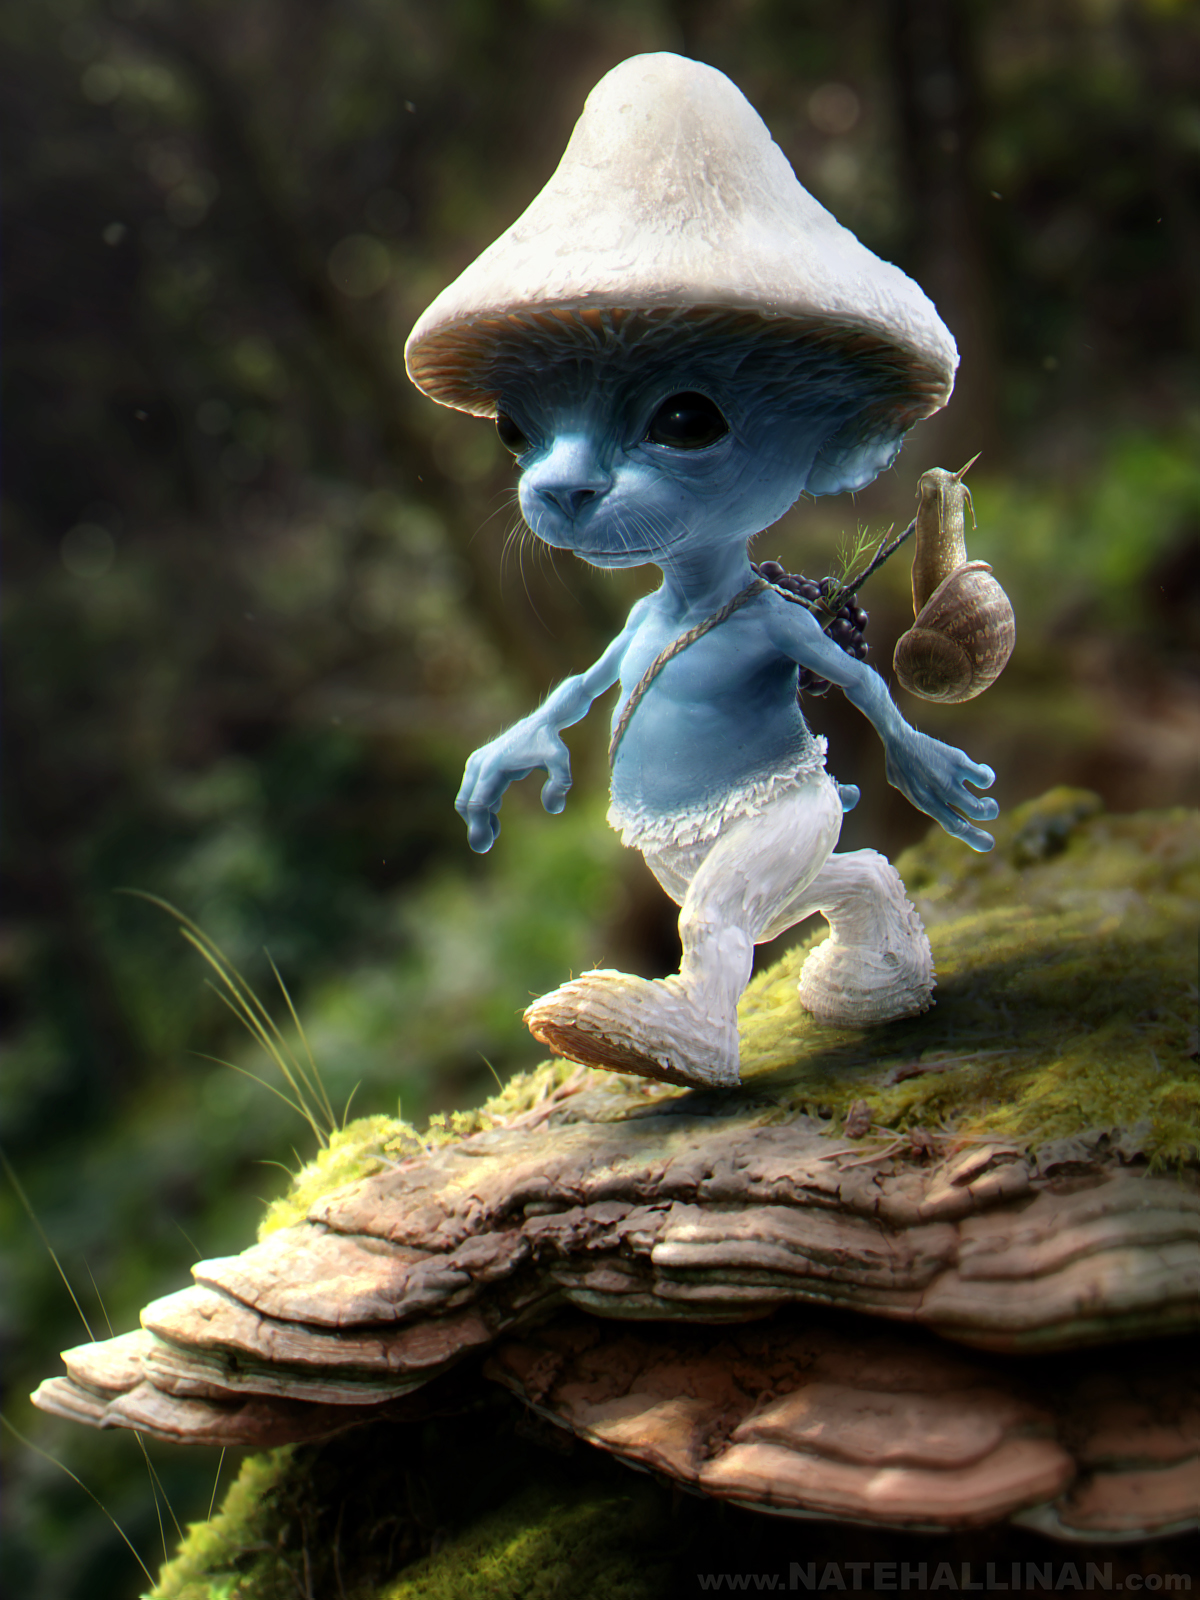
\includegraphics[height=.3in,width=.3in,keepaspectratio]{../images/30.jpg} &
    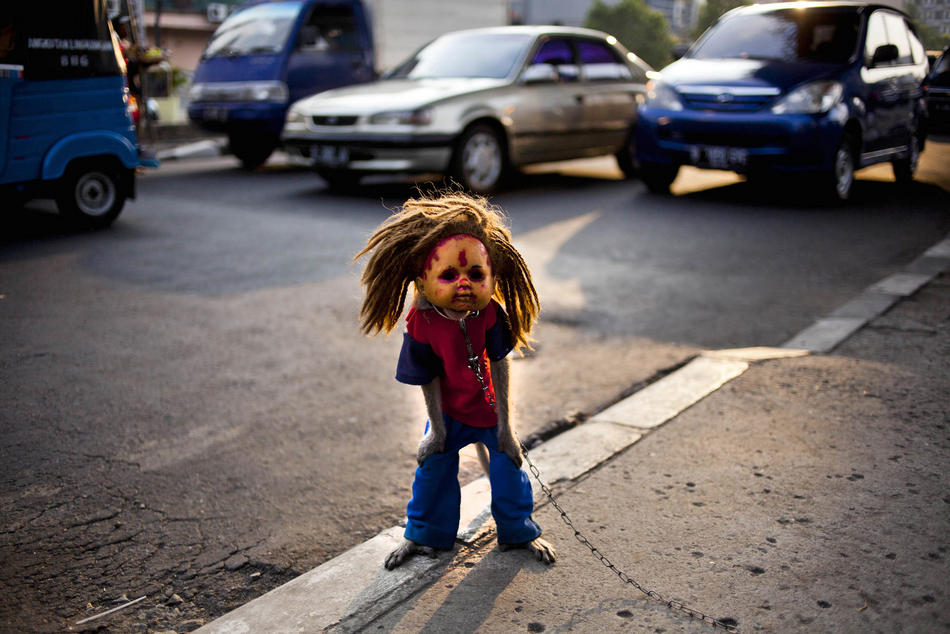
\includegraphics[height=.3in,width=.3in,keepaspectratio]{../images/31.jpg} &
    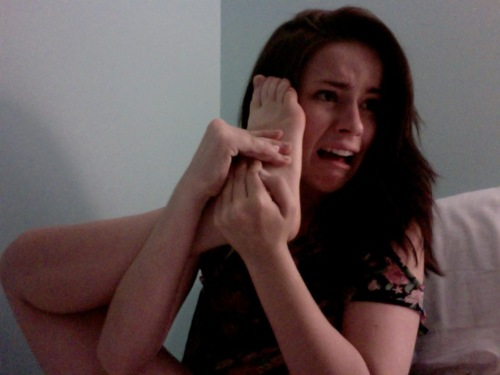
\includegraphics[height=.3in,width=.3in,keepaspectratio]{../images/32.jpg} \\
    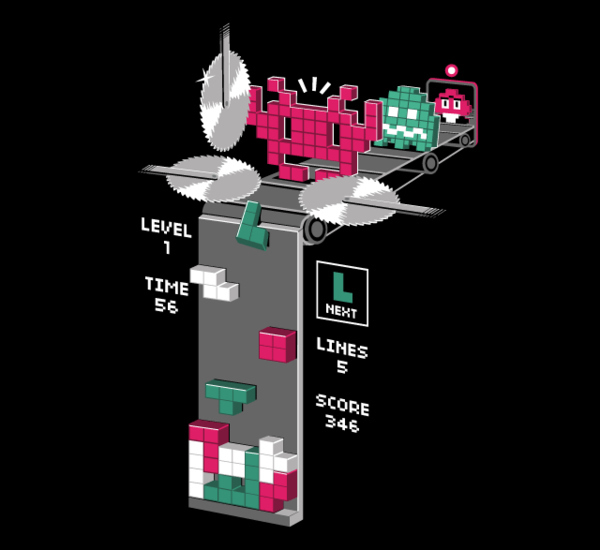
\includegraphics[height=.3in,width=.3in,keepaspectratio]{../images/33.jpg} &
    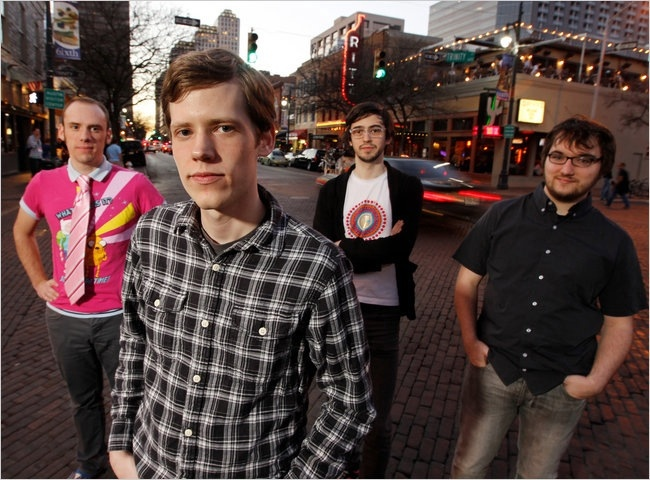
\includegraphics[height=.3in,width=.3in,keepaspectratio]{../images/34.jpg} &
    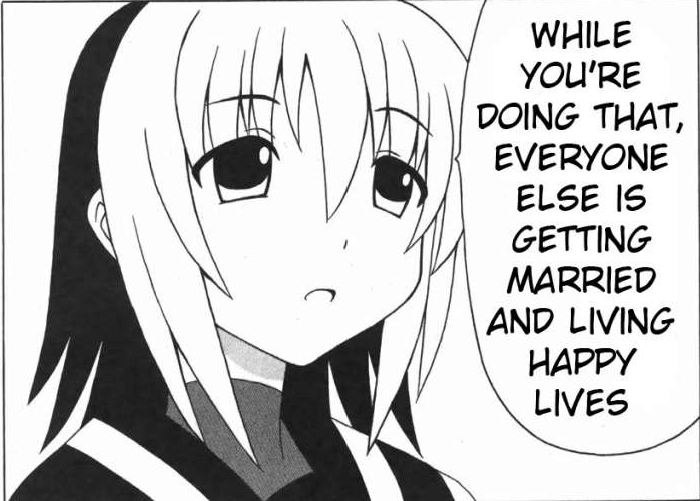
\includegraphics[height=.3in,width=.3in,keepaspectratio]{../images/35.png} &
    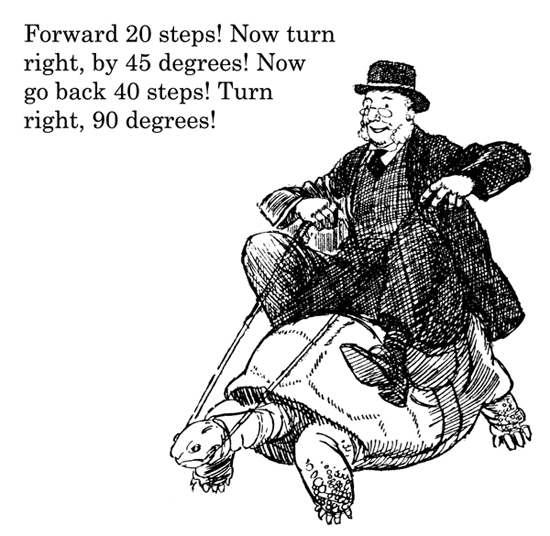
\includegraphics[height=.3in,width=.3in,keepaspectratio]{../images/36.png} &
    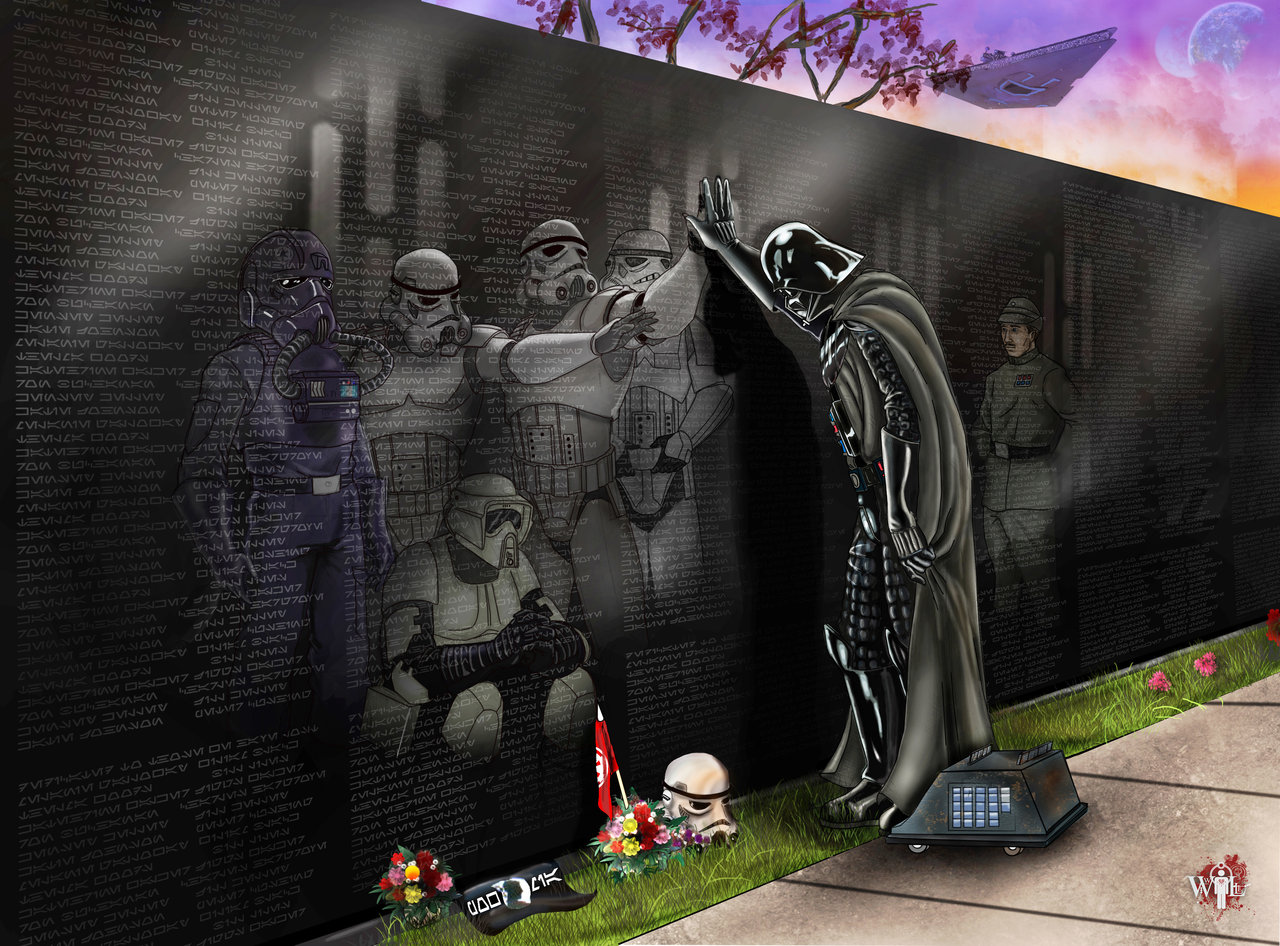
\includegraphics[height=.3in,width=.3in,keepaspectratio]{../images/37.jpg} &
    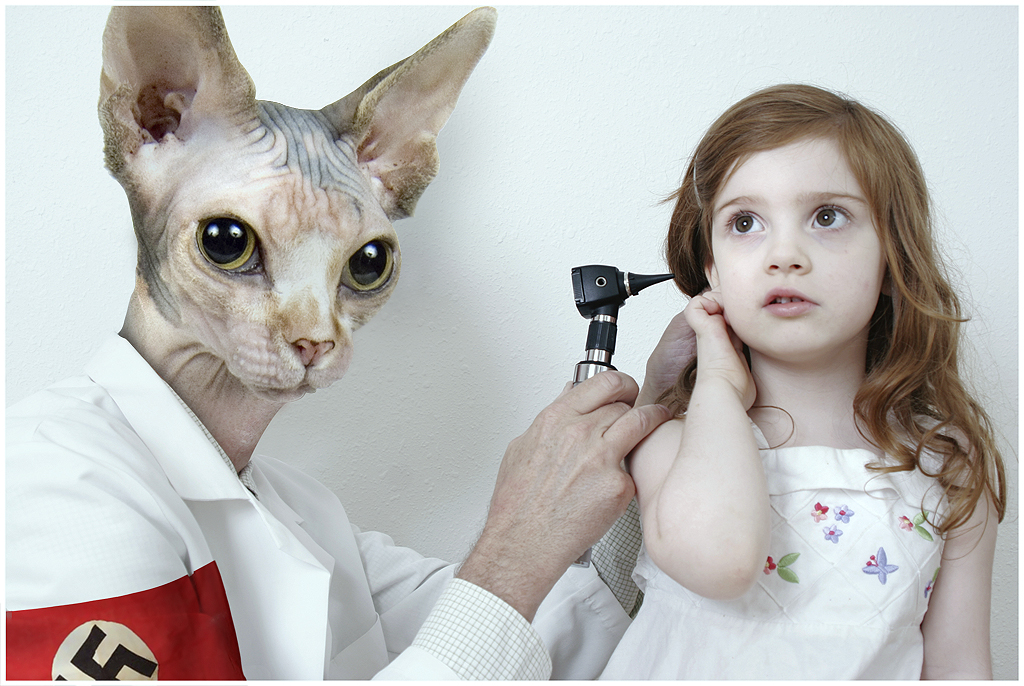
\includegraphics[height=.3in,width=.3in,keepaspectratio]{../images/38.jpg} &
    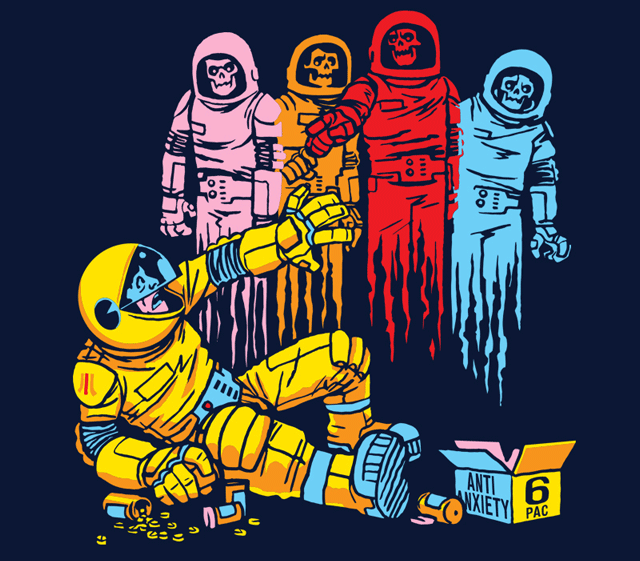
\includegraphics[height=.3in,width=.3in,keepaspectratio]{../images/39.png} &
    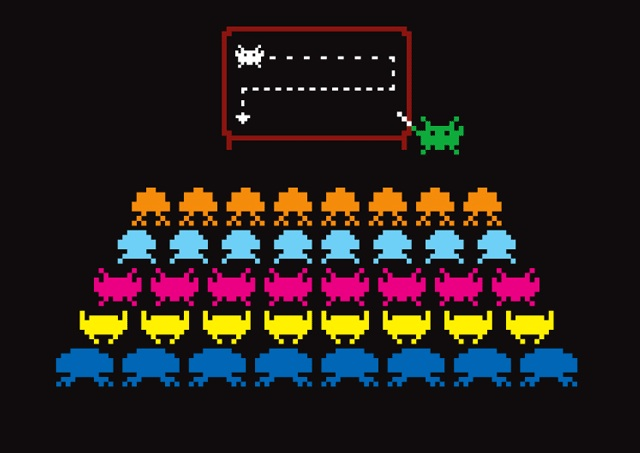
\includegraphics[height=.3in,width=.3in,keepaspectratio]{../images/40.jpg} \\
    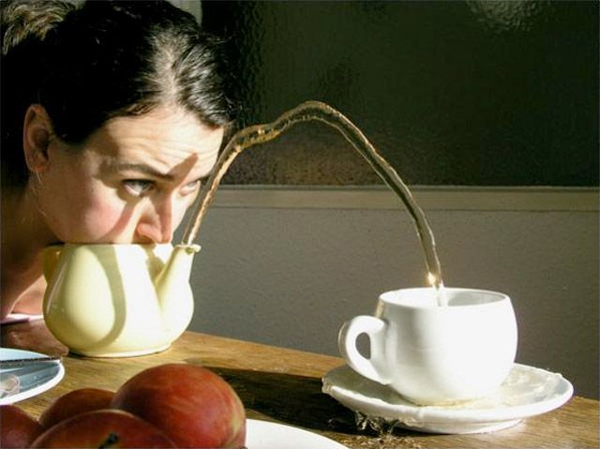
\includegraphics[height=.3in,width=.3in,keepaspectratio]{../images/41.png} &
    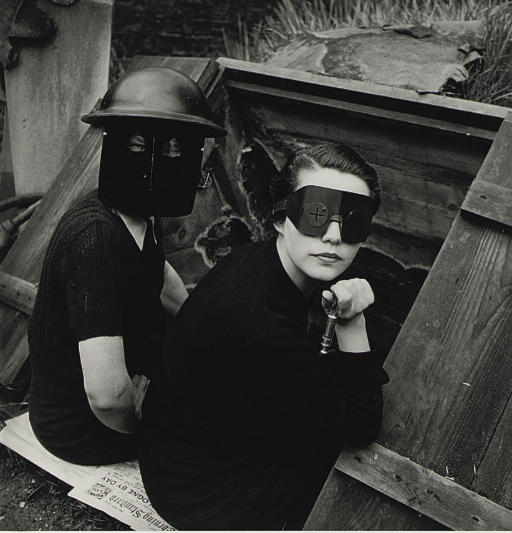
\includegraphics[height=.3in,width=.3in,keepaspectratio]{../images/42.jpg} &
    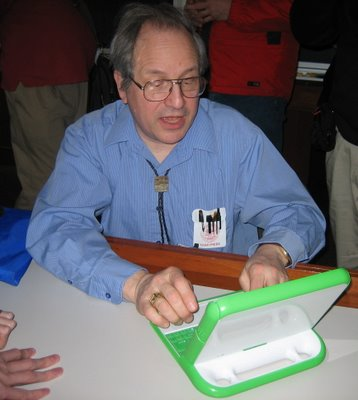
\includegraphics[height=.3in,width=.3in,keepaspectratio]{../images/43.jpg} &
    
\includegraphics[height=.3in,width=.3in,keepaspectratio]{../images/44.jpg} &
    
\includegraphics[height=.3in,width=.3in,keepaspectratio]{../images/45.jpg} &
    
\includegraphics[height=.3in,width=.3in,keepaspectratio]{../images/46.jpg} &
    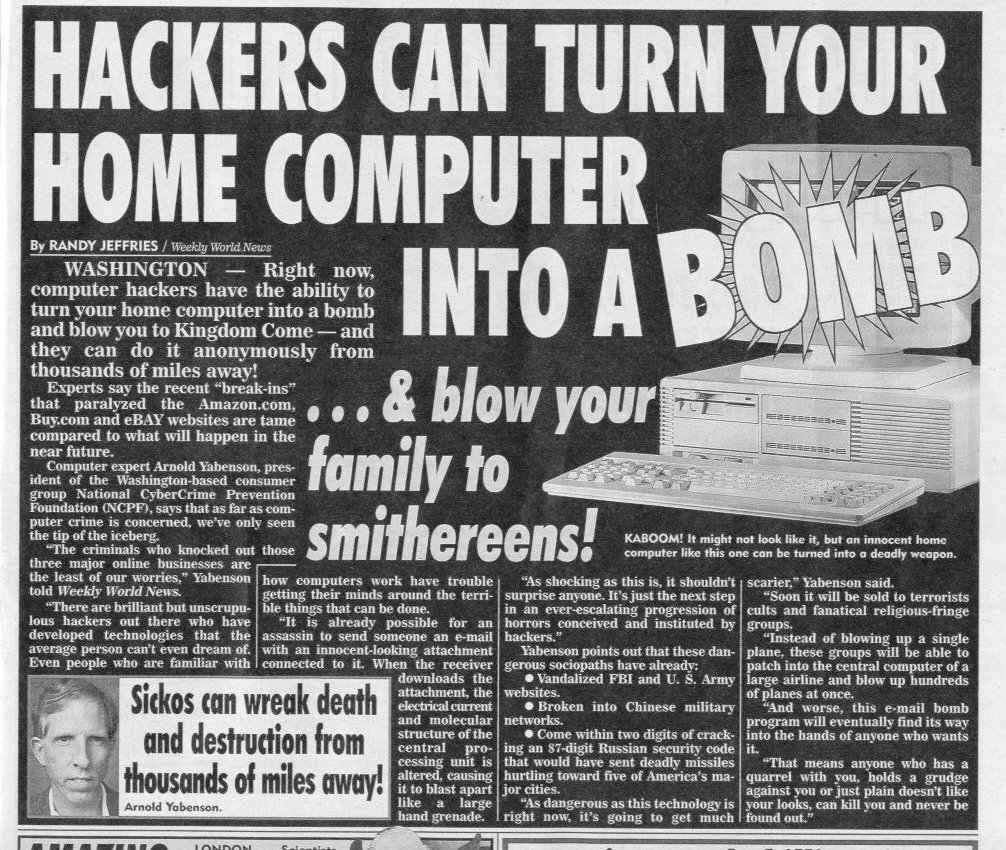
\includegraphics[height=.3in,width=.3in,keepaspectratio]{../images/47.jpg} &
    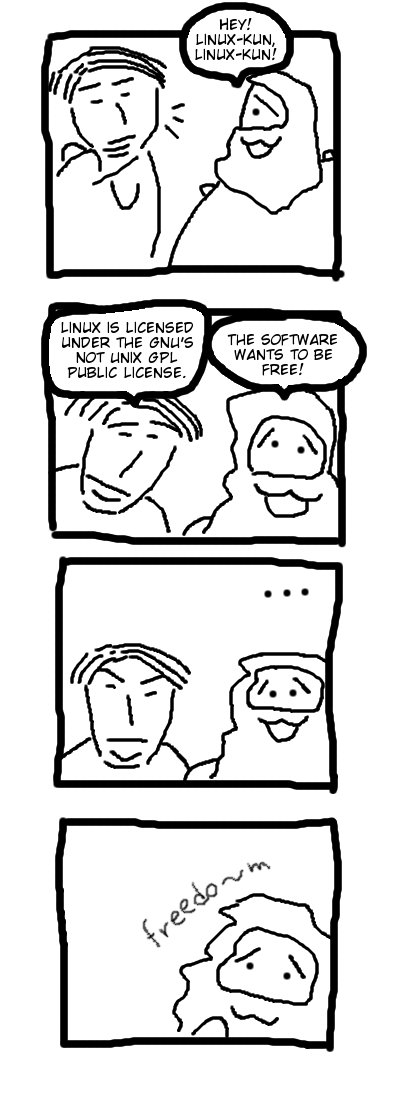
\includegraphics[height=.3in,width=.3in,keepaspectratio]{../images/48.jpg} \\
    \includegraphics[height=.3in,width=.3in,keepaspectratio]{../images/49.jpg} &
    \includegraphics[height=.3in,width=.3in,keepaspectratio]{../images/50.jpg} &
    \includegraphics[height=.3in,width=.3in,keepaspectratio]{../images/51.jpg} &
    \includegraphics[height=.3in,width=.3in,keepaspectratio]{../images/52.png} &
    \includegraphics[height=.3in,width=.3in,keepaspectratio]{../images/53.jpg} &
    \includegraphics[height=.3in,width=.3in,keepaspectratio]{../images/54.jpg} &
    \includegraphics[height=.3in,width=.3in,keepaspectratio]{../images/55.png} &
    \includegraphics[height=.3in,width=.3in,keepaspectratio]{../images/56.jpg} \\
    \includegraphics[height=.3in,width=.3in,keepaspectratio]{../images/57.jpg} &
    \includegraphics[height=.3in,width=.3in,keepaspectratio]{../images/58.jpg} &
    \includegraphics[height=.3in,width=.3in,keepaspectratio]{../images/59.png} &
    \includegraphics[height=.3in,width=.3in,keepaspectratio]{../images/60.png} &
    \includegraphics[height=.3in,width=.3in,keepaspectratio]{../images/61.jpg} &
    \includegraphics[height=.3in,width=.3in,keepaspectratio]{../images/62.jpg} &
    \includegraphics[height=.3in,width=.3in,keepaspectratio]{../images/63.jpg} &
    \includegraphics[height=.3in,width=.3in,keepaspectratio]{../images/64.jpg}
  \end{tabular}

\end{frame}

\begin{frame}
  \frametitle{Ideaal}

  \centering

  Input:

  \includegraphics[scale=.1]{../target.png}

  Output:

  \begin{tabular}{ccccc}
    \includegraphics[scale=.1]{../images/60.png} &
    \includegraphics[scale=.1]{../images/61.jpg} &
    \includegraphics[scale=.1]{../images/62.jpg} &
    \includegraphics[scale=.1]{../images/63.jpg} &
    \includegraphics[scale=.1]{../images/64.jpg}
  \end{tabular}

\end{frame}

\begin{frame}[fragile]
  \frametitle{Vorm}

  \begin{Verbatim}[commandchars=\\\{\}]
\PY{k+kn}{from} \PY{n+nn}{PIL} \PY{k+kn}{import} \PY{n}{Image}
\PY{k+kn}{from} \PY{n+nn}{glob} \PY{k+kn}{import} \PY{n}{glob}

\PY{n}{target} \PY{o}{=} \PY{n}{phash}\PY{p}{(}\PY{n}{Image}\PY{o}{.}\PY{n}{open}\PY{p}{(}\PY{l+s}{'}\PY{l+s}{target.png}\PY{l+s}{'}\PY{p}{)}\PY{p}{)}

\PY{n}{candidates} \PY{o}{=} \PY{n}{glob}\PY{p}{(}\PY{l+s}{'}\PY{l+s}{../images/[0-9][0-9].*}\PY{l+s}{'}\PY{p}{)}
\PY{n}{candidates} \PY{o}{=} \PY{n+nb}{dict}\PY{p}{(}\PY{p}{(}\PY{n}{f}\PY{p}{,} \PY{n}{phash}\PY{p}{(}\PY{n}{Image}\PY{o}{.}\PY{n}{open}\PY{p}{(}\PY{n}{f}\PY{p}{)}\PY{p}{)}\PY{p}{)} \PYZbs{}
                    \PY{k}{for} \PY{n}{f} \PY{o+ow}{in} \PY{n}{candidates}\PY{p}{)}

\PY{n}{diffs} \PY{o}{=} \PY{n+nb}{dict}\PY{p}{(}\PY{p}{)}
\PY{k}{for} \PY{n}{c} \PY{o+ow}{in} \PY{n}{candidates}\PY{p}{:}
    \PY{n}{diffs}\PY{p}{[}\PY{n}{c}\PY{p}{]} \PY{o}{=} \PY{n}{diff}\PY{p}{(}\PY{n}{target}\PY{p}{,} \PY{n}{candidates}\PY{p}{[}\PY{n}{c}\PY{p}{]}\PY{p}{)}

\PY{k}{for} \PY{n}{c} \PY{o+ow}{in} \PY{n+nb}{sorted}\PY{p}{(}\PY{n}{diffs}\PY{p}{,} \PY{n}{key}\PY{o}{=}\PY{n}{diffs}\PY{o}{.}\PY{n}{\PYZus{}\PYZus{}getitem\PYZus{}\PYZus{}}\PY{p}{)}\PY{p}{:}
    \PY{k}{print} \PY{n}{c}\PY{p}{,} \PY{n}{diffs}\PY{p}{[}\PY{n}{c}\PY{p}{]}
\end{Verbatim}


\end{frame}


%% Colour histogram

\begin{frame}
  \frametitle{Eerste poging: kleurenhistogram}

  \begin{itemize}
    \pause \item Probleem:

    \begin{center}
      \includegraphics[scale=.1]{../images/59.png} 
      \hspace{.2in}
      \includegraphics[scale=.2]{../images/59.png}
    \end{center}

    \pause \item Probleem: veel te veel informatie

    \pause

    \begin{center}
      \includegraphics[scale=.2]{../images/41.png}
      \raisebox{.58in}{$\Longrightarrow$}
      \includegraphics[scale=.2]{posterized.png}
    \end{center}
  \end{itemize}
\end{frame}

\begin{frame}[fragile]
  \frametitle{Gemakkelijk!}

  \begin{Verbatim}[commandchars=\\\{\}]
\PY{k}{def} \PY{n+nf}{phash}\PY{p}{(}\PY{n}{im}\PY{p}{)}\PY{p}{:}
    \PY{n}{im} \PY{o}{=} \PY{n}{im}\PY{o}{.}\PY{n}{resize}\PY{p}{(}\PY{p}{(}\PY{l+m+mi}{100}\PY{p}{,} \PY{l+m+mi}{100}\PY{p}{)}\PY{p}{)}\PY{o}{.}\PY{n}{convert}\PY{p}{(}\PY{l+s}{'}\PY{l+s}{P}\PY{l+s}{'}\PY{p}{)}
    \PY{k}{return} \PY{n}{im}\PY{o}{.}\PY{n}{histogram}\PY{p}{(}\PY{p}{)}
\end{Verbatim}


  \pause

  \begin{Verbatim}[commandchars=\\\{\}]
\PY{k}{def} \PY{n+nf}{diff}\PY{p}{(}\PY{n}{h1}\PY{p}{,} \PY{n}{h2}\PY{p}{)}\PY{p}{:}
    \PY{n}{acc} \PY{o}{=} \PY{l+m+mi}{0}
    \PY{k}{for} \PY{n}{a}\PY{p}{,} \PY{n}{b} \PY{o+ow}{in} \PY{n+nb}{zip}\PY{p}{(}\PY{n}{h1}\PY{p}{,} \PY{n}{h2}\PY{p}{)}\PY{p}{:}
        \PY{n}{acc} \PY{o}{+}\PY{o}{=} \PY{n+nb}{abs}\PY{p}{(}\PY{n}{a} \PY{o}{-} \PY{n}{b}\PY{p}{)}
    \PY{k}{return} \PY{n}{acc}
\end{Verbatim}


\end{frame}

\begin{frame}
  \frametitle{Resultaat}

  \centering

  \begin{tabular}{ccc}
    \includegraphics[height=1in,width=1in,keepaspectratio]{../images/60.png} &
    \includegraphics[height=1in,width=1in,keepaspectratio]{../images/64.jpg} &
    \includegraphics[height=1in,width=1in,keepaspectratio]{../images/61.jpg} \\
    0 & 382 & 1594 \\&&\\
    \includegraphics[height=1in,width=1in,keepaspectratio]{../images/63.jpg} &
    \includegraphics[height=1in,width=1in,keepaspectratio]{../images/57.jpg} &
    \includegraphics[height=1in,width=1in,keepaspectratio]{../images/12.jpg} \\
    13762 & 13826 & 13830
  \end{tabular}

\end{frame}


%% Average hash

\begin{frame}
  \frametitle{Tweede poging: average hash}

  \begin{itemize}
    \pause \item Kleuren zijn minder informatief dan vormen

    \pause

    \begin{center}
      \includegraphics[height=1in]{../target.png}
      \raisebox{.48in}{$\Longrightarrow$}
      \includegraphics[height=1in]{bw.png}
    \end{center}

    \pause \item Nog te gevoelig voor details

    \pause

    \begin{center}
      \includegraphics[height=1in]{bw.png}
      \raisebox{.48in}{$\Longrightarrow$}
      \includegraphics[height=1in]{bw_small.png}
    \end{center}
  \end{itemize}
\end{frame}

\begin{frame}[fragile]
  \frametitle{Gemakkelijk!}

  \begin{Verbatim}[commandchars=\\\{\}]
\PY{k}{def} \PY{n+nf}{phash}\PY{p}{(}\PY{n}{im}\PY{p}{)}\PY{p}{:}
    \PY{n}{im} \PY{o}{=} \PY{n}{im}\PY{o}{.}\PY{n}{resize}\PY{p}{(}\PY{p}{(}\PY{l+m+mi}{8}\PY{p}{,} \PY{l+m+mi}{8}\PY{p}{)}\PY{p}{)}\PY{o}{.}\PY{n}{convert}\PY{p}{(}\PY{l+s}{'}\PY{l+s}{L}\PY{l+s}{'}\PY{p}{)}
    \PY{n}{avg} \PY{o}{=} \PY{n+nb}{sum}\PY{p}{(}\PY{n}{im}\PY{o}{.}\PY{n}{getdata}\PY{p}{(}\PY{p}{)}\PY{p}{)} \PY{o}{/} \PY{l+m+mf}{64.}
    \PY{n}{data} \PY{o}{=} \PY{n+nb}{map}\PY{p}{(}\PY{k}{lambda} \PY{n}{i}\PY{p}{:} \PY{l+m+mi}{0} \PY{k}{if} \PY{n}{i} \PY{o}{<} \PY{n}{avg} \PY{k}{else} \PY{l+m+mi}{1}\PY{p}{,}
               \PY{n}{im}\PY{o}{.}\PY{n}{getdata}\PY{p}{(}\PY{p}{)}\PY{p}{)}
    \PY{k}{return} \PY{n+nb}{reduce}\PY{p}{(}\PY{k}{lambda} \PY{n}{x}\PY{p}{,} \PY{p}{(}\PY{n}{y}\PY{p}{,} \PY{n}{z}\PY{p}{)}\PY{p}{:} \PY{n}{x} \PY{o}{|} \PY{p}{(}\PY{n}{z} \PY{o}{<<} \PY{n}{y}\PY{p}{)}\PY{p}{,}
                  \PY{n+nb}{enumerate}\PY{p}{(}\PY{n}{data}\PY{p}{)}\PY{p}{,}
                  \PY{l+m+mi}{0}\PY{p}{)}
\end{Verbatim}


  \pause

  \begin{Verbatim}[commandchars=\\\{\}]
\PY{k}{def} \PY{n+nf}{diff}\PY{p}{(}\PY{n}{h1}\PY{p}{,} \PY{n}{h2}\PY{p}{)}\PY{p}{:}
    \PY{n}{h}\PY{p}{,} \PY{n}{d} \PY{o}{=} \PY{l+m+mi}{0}\PY{p}{,} \PY{n}{h1} \PY{o}{\PYZca{}} \PY{n}{h2}
    \PY{k}{while} \PY{n}{d}\PY{p}{:}
        \PY{n}{h} \PY{o}{+}\PY{o}{=} \PY{l+m+mi}{1}
        \PY{n}{d} \PY{o}{&}\PY{o}{=} \PY{n}{d} \PY{o}{-} \PY{l+m+mi}{1}
    \PY{k}{return} \PY{n}{h}
\end{Verbatim}


\end{frame}

\begin{frame}
  \frametitle{Resultaat}

  \centering

  \begin{tabular}{ccc}
    \includegraphics[height=1in,width=1in,keepaspectratio]{../images/60.png} &
    \includegraphics[height=1in,width=1in,keepaspectratio]{../images/61.jpg} &
    \includegraphics[height=1in,width=1in,keepaspectratio]{../images/64.jpg} \\
    0 & 0 & 0 \\&&\\
    \includegraphics[height=1in,width=1in,keepaspectratio]{../images/62.jpg} &
    \includegraphics[height=1in,width=1in,keepaspectratio]{../images/25.jpg} &
    \includegraphics[height=1in,width=1in,keepaspectratio]{../images/31.jpg} \\
    0 & 26 & 26
  \end{tabular}

\end{frame}


%% Discrete cosine transform

\begin{frame}
  \frametitle{Derde poging: discrete cosine transform}

  \pause

  {\bf Drukt een reeks datapoints uit als de som van cosinusfuncties van
       verschillende frequenties}

  \begin{itemize}
    \pause \item Ook gebruikt in JPEG (en MP3)
    \pause \item Laat ons toe de kleine hoge-frequentie componenten te laten
                 vallen
  \end{itemize}
\end{frame}

\begin{frame}[fragile]
  \frametitle{Gemakkelijk?}

  \begin{Verbatim}[commandchars=\\\{\}]
\PY{k+kn}{import} \PY{n+nn}{math}

\PY{k}{def} \PY{n+nf}{phash}\PY{p}{(}\PY{n}{im}\PY{p}{)}\PY{p}{:}
    \PY{n}{im} \PY{o}{=} \PY{n}{im}\PY{o}{.}\PY{n}{resize}\PY{p}{(}\PY{p}{(}\PY{l+m+mi}{32}\PY{p}{,} \PY{l+m+mi}{32}\PY{p}{)}\PY{p}{)}\PY{o}{.}\PY{n}{convert}\PY{p}{(}\PY{l+s}{'}\PY{l+s}{L}\PY{l+s}{'}\PY{p}{)}
    \PY{n}{seq} \PY{o}{=} \PY{p}{[}\PY{n+nb}{sum}\PY{p}{(}\PY{n}{im}\PY{o}{.}\PY{n}{getpixel}\PY{p}{(}\PY{p}{(}\PY{n}{x}\PY{p}{,} \PY{n}{y}\PY{p}{)}\PY{p}{)} \PY{o}{*}
               \PY{n}{math}\PY{o}{.}\PY{n}{cos}\PY{p}{(}\PY{n}{math}\PY{o}{.}\PY{n}{pi} \PY{o}{/} \PY{l+m+mi}{32} \PY{o}{*} \PY{p}{(}\PY{n}{x} \PY{o}{+} \PY{o}{.}\PY{l+m+mi}{5}\PY{p}{)} \PY{o}{*} \PY{n}{u}\PY{p}{)} \PY{o}{*}
               \PY{n}{math}\PY{o}{.}\PY{n}{cos}\PY{p}{(}\PY{n}{math}\PY{o}{.}\PY{n}{pi} \PY{o}{/} \PY{l+m+mi}{32} \PY{o}{*} \PY{p}{(}\PY{n}{y} \PY{o}{+} \PY{o}{.}\PY{l+m+mi}{5}\PY{p}{)} \PY{o}{*} \PY{n}{v}\PY{p}{)}
               \PY{k}{for} \PY{n}{x} \PY{o+ow}{in} \PY{n+nb}{range}\PY{p}{(}\PY{l+m+mi}{32}\PY{p}{)} \PY{k}{for} \PY{n}{y} \PY{o+ow}{in} \PY{n+nb}{range}\PY{p}{(}\PY{l+m+mi}{32}\PY{p}{)}\PY{p}{)}
           \PY{k}{for} \PY{n}{v} \PY{o+ow}{in} \PY{n+nb}{range}\PY{p}{(}\PY{l+m+mi}{8}\PY{p}{)} \PY{k}{for} \PY{n}{u} \PY{o+ow}{in} \PY{n+nb}{range}\PY{p}{(}\PY{l+m+mi}{8}\PY{p}{)}\PY{p}{]}
    \PY{n}{avg} \PY{o}{=} \PY{n+nb}{sum}\PY{p}{(}\PY{n}{seq}\PY{p}{[}\PY{l+m+mi}{1}\PY{p}{:}\PY{p}{]}\PY{p}{)} \PY{o}{/} \PY{p}{(}\PY{n+nb}{len}\PY{p}{(}\PY{n}{seq}\PY{p}{)} \PY{o}{-} \PY{l+m+mi}{1}\PY{p}{)}
    \PY{n}{data} \PY{o}{=} \PY{n+nb}{map}\PY{p}{(}\PY{k}{lambda} \PY{n}{i}\PY{p}{:} \PY{l+m+mi}{0} \PY{k}{if} \PY{n}{i} \PY{o}{<} \PY{n}{avg} \PY{k}{else} \PY{l+m+mi}{1}\PY{p}{,} \PY{n}{seq}\PY{p}{)}
    \PY{k}{return} \PY{n+nb}{reduce}\PY{p}{(}\PY{k}{lambda} \PY{n}{x}\PY{p}{,} \PY{p}{(}\PY{n}{y}\PY{p}{,} \PY{n}{z}\PY{p}{)}\PY{p}{:} \PY{n}{x} \PY{o}{|} \PY{p}{(}\PY{n}{z} \PY{o}{<<} \PY{n}{y}\PY{p}{)}\PY{p}{,}
                  \PY{n+nb}{enumerate}\PY{p}{(}\PY{n+nb}{map}\PY{p}{(}\PY{n}{data}\PY{p}{)}\PY{p}{,}
                  \PY{l+m+mi}{0}\PY{p}{)}
\end{Verbatim}


\end{frame}

\begin{frame}
  \frametitle{Resultaat}

  \centering

  \begin{tabular}{ccc}
    \includegraphics[height=1in,width=1in,keepaspectratio]{../images/60.png} &
    \includegraphics[height=1in,width=1in,keepaspectratio]{../images/62.jpg} &
    \includegraphics[height=1in,width=1in,keepaspectratio]{../images/61.jpg} \\
    0 & 0 & 2 \\&&\\
    \includegraphics[height=1in,width=1in,keepaspectratio]{../images/64.jpg} &
    \includegraphics[height=1in,width=1in,keepaspectratio]{../images/63.jpg} &
    \includegraphics[height=1in,width=1in,keepaspectratio]{../images/32.jpg} \\
    4 & 22 & 23
  \end{tabular}

\end{frame}


%% Extro

\begin{frame}
  \frametitle{Oefeningen voor thuis}

  \centering

  \begin{tabular}{cc}
    Rotatie? & Reflectie? \\
    \includegraphics[scale=.25,angle=90]{../target.png} &
    \reflectbox{\includegraphics[scale=.25]{../target.png}}
  \end{tabular}

  \pause Nodig?

\end{frame}

\begin{frame}
  \frametitle{Nogmaals}

  Alle code, afbeeldingen, slides:

  \centering

  \LARGE \url{https://github.com/Cairnarvon/phash-presentation}

\end{frame}

\end{document}
